\documentclass[11pt]{charter}

% El títulos de la memoria, se usa en la carátula y se puede usar el cualquier lugar del documento con el comando \ttitle
\titulo{Multi potenciostato} 

% Nombre del posgrado, se usa en la carátula y se puede usar el cualquier lugar del documento con el comando \degreename
\posgrado{Carrera de Especialización en Sistemas Embebidos} 
%\posgrado{Carrera de Especialización en Internet de las Cosas} 
%\posgrado{Carrera de Especialización en Intelegencia Artificial}
%\posgrado{Maestría en Sistemas Embebidos} 
%\posgrado{Maestría en Internet de las cosas}

% Tu nombre, se puede usar el cualquier lugar del documento con el comando \authorname
\autor{Fabiola de las Casas Escardó} 

% El nombre del director y co-director, se puede usar el cualquier lugar del documento con el comando \supname y \cosupname y \pertesupname y \pertecosupname
\director{Juan Manuel Reta}
\pertenenciaDirector{UNER} 
% FIXME:NO IMPLEMENTADO EL CODIRECTOR ni su pertenencia
\codirector{Eduardo Filomena} % si queda vacio no se deberíá incluir 
\pertenenciaCoDirector{UNER}

% Nombre del cliente, quien va a aprobar los resultados del proyecto, se puede usar con el comando \clientename y \empclientename
\cliente{Guido Rozenblum}
\empresaCliente{Aplife Biotech S.A.}

% Nombre y pertenencia de los jurados, se pueden usar el cualquier lugar del documento con el comando \jurunoname, \jurdosname y \jurtresname y \perteunoname, \pertedosname y \pertetresname.
\juradoUno{Nombre y Apellido (1)}
\pertenenciaJurUno{pertenencia (1)} 
\juradoDos{Nombre y Apellido (2)}
\pertenenciaJurDos{pertenencia (2)}
\juradoTres{Nombre y Apellido (3)}
\pertenenciaJurTres{pertenencia (3)}
 
\fechaINICIO{27 de Junio de 2020}		%Fecha de inicio de la cursada de GdP \fechaInicioName
\fechaFINALPlanificacion{22 de Agosto de 2020} 	%Fecha de final de cursada de GdP
\fechaFINALTrabajo{28 de Mayo de 2021}		%Fecha de defensa pública del trabajo final


\begin{document}

\maketitle
\thispagestyle{empty}
\pagebreak


\thispagestyle{empty}
{\setlength{\parskip}{0pt}
\tableofcontents{}
}
\pagebreak


\section{Registros de cambios}
\label{sec:registro}


\begin{table}[ht]
\label{tab:registro}
\centering

\begin{tabularx}{\linewidth}{@{}|c|X|c|@{}}
\hline
\rowcolor[HTML]{C0C0C0} 
Revisión & \multicolumn{1}{c|}{\cellcolor[HTML]{C0C0C0}Detalles de los cambios realizados} & Fecha      \\ \hline
1.0      & Creación del documento     & 27/06/2020 \\ \hline
1.1      & Se completó hasta el punto 6 inclusive  & 11/07/2020  \\ \hline
1.2      & Se completó hasta el punto 11 inclusive y se realizaron las correcciones indicadas                  & 29/07/2020\\ \hline
\end{tabularx}
\end{table}

\pagebreak



\section{Acta de constitución del proyecto}
\label{sec:acta}

\begin{flushright}
Buenos Aires, \fechaInicioName
\end{flushright}

\vspace{2cm}

Por medio de la presente se acuerda con la Ing. \authorname\hspace{1px} que su Trabajo Final de la \degreename\hspace{1px} se titulará ``\ttitle'', consistirá esencialmente en el prototipo preliminar de un potenciostato de 32 canales para la realización en simultáneo de experimentos electroquímicos, y tendrá un presupuesto preliminar estimado de 660 hs de trabajo, con fecha de inicio \fechaInicioName\hspace{1px} y fecha de presentación pública \fechaFinalName.

Se adjunta a esta acta la planificación inicial.

\vfill

% Esta parte se construye sola con la información que hayan cargado en el preámbulo del documento y no debe modificarla
\begin{table}[ht]
\centering
\begin{tabular}{ccc}
\begin{tabular}[c]{@{}c@{}}Ariel Lutenberg \\ Director posgrado FIUBA\end{tabular} &  & \begin{tabular}[c]{@{}c@{}}\clientename \\ \empclientename \end{tabular} \vspace{2.5cm} \\ 
\multicolumn{3}{c}{\begin{tabular}[c]{@{}c@{}} \supname \\ Director del Trabajo Final \\
\\
\cosupname \\ Co-director del Trabajo Final
\end{tabular}} \vspace{2.5cm} \\
\begin{tabular}[c]{@{}c@{}}\jurunoname \\ Jurado del Trabajo Final\end{tabular}     &  & \begin{tabular}[c]{@{}c@{}}\jurdosname\\ Jurado del Trabajo Final\end{tabular}  \vspace{2.5cm}  \\
\multicolumn{3}{c}{\begin{tabular}[c]{@{}c@{}} \jurtresname\\ Jurado del Trabajo Final\end{tabular}} \vspace{.5cm}                                                                     
\end{tabular}
\end{table}




\section{Descripción técnica-conceptual del proyecto a realizar}
\label{sec:descripcion}

En la actualidad uno de los principales desafíos de la industria farmacéutica y de diagnóstico es la dificultad de encontrar moléculas capaces de actuar como biosensores. Debido a esto existen muy pocos dispositivos que permitan hacer mediciones y detección de patologías \textit{in-situ}, y se debe recurrir normalmente a análisis de laboratorio y procesos largos hasta obtener los resultados del estudio. 

Aplife Biotech es una \textit{startup} argentina que está desarrollando una tecnología para optimizar estos procesos de descubrimiento de moléculas y así lograr dotar a la industria farmacéutica y de diagnóstico con la capacidad de desarrollar dispositivos portátiles que detecten fácil y rápidamente problemas de salud. De esta forma se logrará descentralizar los ensayos de diagnósticos de los principales laboratorios y promoverá su portabilidad. El desarrollo de esta tecnología también puede tener un gran impacto en el medioambiente donde muchas veces es necesaria una detección rápida de patógenos o agentes tóxicos.

El objetivo de este proyecto es el desarrollo de un potenciostato. Esto es un dispositivo que se usa para mediciones de electroquímica. Su funcionamiento principal es aplicar una magnitud física que provoque una reacción química que sea medida por el mismo equipo. Por lo tanto, van a ser los dispositivos encargados de encontrar qué moléculas se comportan mejor como transductor para la detección de cada patología o agente que se desee estudiar. 

El dispositivo a desarrollar tendrá como función principal aplicar un potencial variable en el tiempo y medir la corriente que genera la reacción electroquímica entre una molécula y una solución. Esto se conoce como voltametría. Existen distintos tipos de voltametría y este proyecto se va a centrar en tres: la voltametría cíclica, la cuadrada y la rampa escalonada.
\begin{itemize}
\item \textbf{Voltametría cíclica:} consiste en aplicar una onda triangular y medir la reacción. Esta medición puede ser de máximos y mínimos o de valores en intervalos establecidos por el usuario. También se configuran la altura de la onda triangular y la pendiente.
\item \textbf{Voltametría Cuadrada:} se aplica una onda cuadrada y se mide la reacción. La medición es nuevamente de máximos y mínimos o en un tiempo definido cuando la señal aplicada es máxima y cuando es mínima. Se configura la altura y el \textit{duty cycle}.
\item \textbf{Voltametría rampa escalonada (\textit{SWV: square wave voltammetry}):} es una onda cuadrada montada sobre una onda triangular. La medición se realiza en el 10\% antes que la señal cambie de tensión. Se pueden configurar la pendiente, el duty cycle y las tensiones máximas y mínimas. 
\end{itemize}


Un potenciostato está compuesto por 3 electrodos encargados de aplicar la tensión y tomar las lecturas de interés denominados \textit{Counter Electrode} (CE), \textit{Working Electrode} (WE) y \textit{Reference Electrode} (RE). El CE es el encargado de aplicar la señal y el RE controla que la señal aplicada por el CE sea la esperada. El WE es donde se deposita la molécula que se desea estudiar y, por lo tanto, el encargado de realizar la medición. Los potenciostatos disponibles en el mercado tienen como máximo 16  canales limitando la cantidad de experimentos a realizar en simultáneo y prolongando su tiempo de los mismos. 

El equipo actual que posee Aplife Biotech S.A. cuenta con 10 canales, 4 ADC, 1 DAC y todo es controlado por un microcontrolador de 8 bits. La empresa busca mejorar este prototipo aumentando la cantidad de canales a 32, mejorando la interfaz con el usuario mediante comunicación USB, permitiendo un almacenamiento interno de los datos obtenidos en las mediciones y realizando el control mediante una FPGA. Esto se debe a que se busca que el potenciostato final sea un ASIC para así lograr agrupar una mayor cantidad de electrodos en un espacio menor y de esta forma masificar las mediciones. Estos ASIC van a necesitar un dispositivo donde sean conectados y puedan ser controlados. Por esta razón, como se muestra en la Figura \ref{fig:diagBloques}, se va a dividir el proyecto en dos partes: el potenciostato y el dispositivo de control. En la misma se muestra un único conjunto de electrodos de forma representativa.

\begin{figure}[!ht]
\centering 
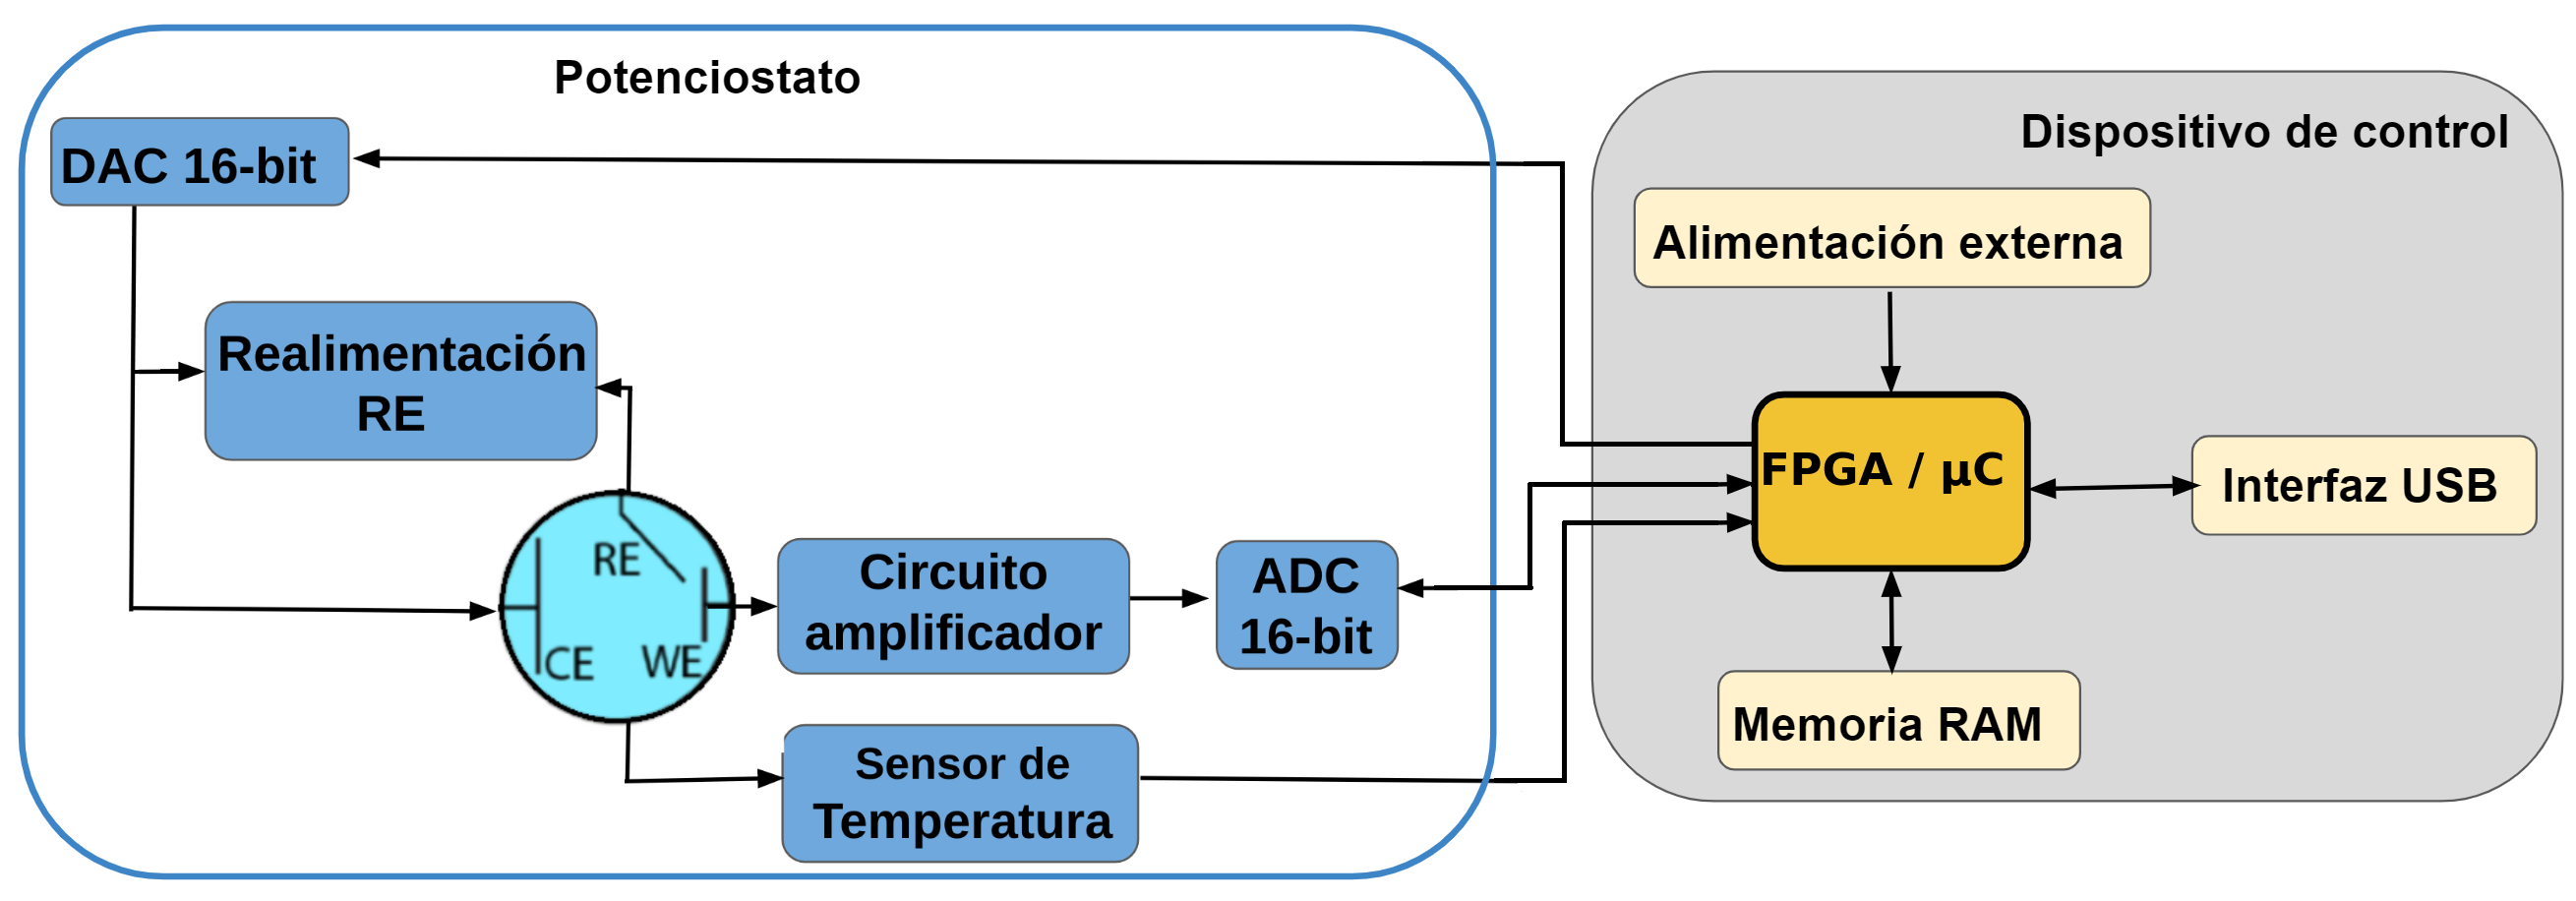
\includegraphics[width=1\textwidth]{./Figuras/diagrama_bloques.png}
\caption{Diagrama en bloques del sistema}
\label{fig:diagBloques}
\end{figure}

El bloque del potenciostato consta de un sensor de temperatura, un DAC de 16 bits encargado de aplicar la señal seleccionada por el usuario y un ADC de 16 bits para la adquisición de datos. La señal analógica del DAC se aplica al CE mediante un circuito de realimentación cuya señal de control será tomada por el electrodo RE. Esta señal desencadena una reacción química en el electrodo WE que genera una corriente. Esta corriente puede ir desde los pA a los 100 nA, por lo que es necesario un circuito de amplificación previo a hacer la conversión AD. Este debe poder ser manipulado por la FPGA para seleccionar el multiplicador adecuado para tener una correcta lectura en el ADC.
 
El dispositivo de control gira en torno a una FPGA. La interfaz USB permite al usuario configurar la señal que quiere aplicar y ver los datos del experimento resultante desde cualquier PC mediante una aplicación UI. Además el FPGA debe procesar la información adquirida del ADC y del sensor de temperatura y almacenarla en una memoria RAM externa, para después transmitirla a la PC.


\section{Identificación y análisis de los interesados}
\label{sec:interesados}


\begin{table}[H]
%\caption{Identificación de los interesados}
%\label{tab:interesados}
\begin{tabularx}{\linewidth}{@{}|l|X|X|l|@{}}
\hline
\rowcolor[HTML]{C0C0C0} 
Rol           & Nombre y Apellido & Organización 	& Puesto 	\\ \hline
Cliente       & \clientename      &\empclientename	& CTO     	\\ \hline
Responsable   & \authorname       & \empclientename & Ingeniera de Desarrollo \\ \hline
Colaboradores & Iván G. Politzer  &\empclientename	& Ingeniero de Desarrollo  	\\ \hline
%Orientador    & \supname  & \pertesupname	& Director	Trabajo final \\ \hline
\multicolumn{1}{|c|}{} & \supname     & \pertesupname   & Director del Trabajo final \\ \cline{2-4} 
\multicolumn{1}{|c|}{\multirow{-2}{*}{Orientadores}} & \cosupname  & \pertesupname  & Co-director del Trabajo final \\ \hline
Usuario final & Biólogos y Biotecnólogos         &\empclientename 	&  -      	\\ \hline
\end{tabularx}
\end{table}

\section{1. Propósito del proyecto}
\label{sec:proposito}

El próposito de este proyecto es desarrollar un prototipo funcional de un potenciostato de múltiples canales que pueda realizar distintos tipos de pruebas de voltimetría y adquirir los datos de las reacciones electroquímicas que se produzcan. 


\section{2. Alcance del proyecto}
\label{sec:alcance}

El presente proyecto incluye:
\begin{itemize}
\item Prototipo funcional.
\item Desarrollo y documentación de firmware.
\item Desarrollo de PCB para bloque de potenciostato.
\item Documentación de hardware.
\item Programa en python para graficar las mediciones obtenidas.  
\item Pruebas de validación y verificación.
\end{itemize}

El presente proyecto no incluye:
\begin{itemize}
\item Desarrollo de una aplicación de PC para interfaz de usuario, el sistema debe ser controlado por línea de comando.
\item Fabricación del PCB de dispositivo de control, que se realizará con una placa de desarrollo de la marca elegida.
\item Gabinete.
\end{itemize}


\section{3. Supuestos del proyecto}
\label{sec:supuestos}
Para el desarrollo del presente proyecto se supone que:
\begin{itemize}
\item Los fondos estipulados estarán disponibles para la duración del proyecto.
\item El tiempo para el desarrollo será suficiente.
\item No surgirá ningún proyecto de mayor importancia en la empresa.
\item Los materiales necesarios serán adquiridos en tiempo y forma.
\end{itemize}

\section{4. Requerimientos}
\label{sec:requerimientos}

\begin{enumerate}

\item \textbf{Requerimientos generales del proyecto:}
\begin{enumerate}
	\item Debe poder controlarse mediante USB 3.1
	\item La documentación del proyecto debe seguirse con control de versiones GIT.
\end{enumerate}

\item \textbf{Requerimientos de mediciones:}
\begin{enumerate}
	\item Se deben poder medir corrientes en el rango de 1 pA hasta los 100 nA. Rango previamente definido por el usuario.
	\item El error de las mediciones, una vez seleccionado el rango de corriente, debe ser menor al 10\%
	\item Todos los electrodos se tienen que poder medir en 1,6 ms o a una frecuencia de 625Hz.
	\item Se debe poder seleccionar si medir mínimos y máximos o tomar mediciones en intervalos de tiempo constantes y definidos por el usuario.
\end{enumerate}

\item \textbf{Requerimientos de voltametría:}
\begin{enumerate}
	\item El DAC debe tener un rango de \underline{+}1,5 V
	\item Voltametría cíclica
	\begin{enumerate}
		\item Se debe poder seleccionar la pendiente entre 10 mV/s a 1 V/s 
	\end{enumerate}
	\item Voltametría cuadrada y rampa escalonada
	\begin{enumerate}
		\item El \textit{duty cycle} deber ser del 50\%
		\item La altura de los saltos de tensión deben ser configurables
		\item La medición se debe realizar en el ultimo 10\% del ancho de los pulsos antes de cambiar de estado.
	\end{enumerate}
\end{enumerate}

\item \textbf{Requerimientos de hardware:}
\begin{enumerate}
	\item Los electrodos deben estar recubiertos de oro y serán provistos por la empresa.
	\item Los electrodos deben estar en un PCB separado para que puedan ser conectados y desconectados al potenciostato.
\end{enumerate}

\end{enumerate}

\section{5. Historias de usuarios (\textit{Product backlog})}
\label{sec:backlog}

\section{6. Entregables principales del proyecto}
\label{sec:entregables}

\begin{itemize}
\item Equipo funcionando
\item Manual de uso
\item Código fuente
\item Informe final

\end{itemize}


\section{7. Desglose del trabajo en tareas}
\label{sec:wbs}

\begin{enumerate}
\item \textbf{Análisis preliminar (40 hs hs)} 
	\begin{enumerate}
		\item Definición del alcance del proyecto (8 hs)
		\item Definición de requerimientos (10 hs)
		\item Planificación (6 hs)
		\item Bibliografía de experimentos de voltametría (16 hs)
	\end{enumerate}
\item \textbf{Diseño y construcción de hardware - Potenciostato (60 hs)}
	\begin{enumerate}
		\item Revisión y re-diseño del circuito actual (8 hs)
		\item Definición de circuito para la selección de amplificación pre conversor AD (10 hs)
		\item Selección de componentes (10 hs)
		\item Adquisición de componentes (2 hs)
		\item Pruebas básicas de comportamiento del circuito (16 hs)
		\item Desarrollo del PCB (8 hs)
		\item Montaje del prototipo en el PCB (4 hs)
		\item Documentación (2 hs)
	\end{enumerate}
\item \textbf{Diseño y construcción de hardware - Dispositivo de control (124 hs)}
	\begin{enumerate}
		\item Estudio y selección de placa de desarrollo de FPGA (24 hs)
		\item Estudio y selección de memoria RAM (24 hs)
		\item Selección de tipo de alimentación externa (12 hs)
		\item Adquisición de componentes elegidos (2 hs)
		\item Pruebas iniciales en placa de desarrollo (36 hs)
		\item Pruebas de potencia de alimentación externa (24 hs)
		\item Documentación (2 hs)
	\end{enumerate}
\item \textbf{Desarrollo de firmware (206 hs)}
	\begin{enumerate}
		\item Driver conversor DA (36 hs)
		\item Driver conversor AD (36 hs)
		\item Driver de sensor de temperatura (24 hs)
		\item Almacenamiento en memoria externa RAM (40 hs)
		\item Comunicación USB (36 hs)
		\item Módulo para la selección del circuito amplificador (24 hs)	
		\item Integración de firmware (8 hs)
		\item Documentación (2 hs)
	\end{enumerate}		
\item \textbf{Validación y Verificación (160 hs)}
	\begin{enumerate}
		\item Validación y verificación de señales aplicadas con el conversor DA (24 hs)
		\item Validación y verificación de almacenamiento en memoria RAM externa (24 hs)
		\item Validación y verificación de sensor de temperatura (24 hs)
		\item Pruebas con soluciones electroquímicas conocidas (44 hs)
		\item Ajustes de parámetros a partir de los resultados obtenidos en las pruebas (36 hs)
		\item Documentación (8 hs)
	\end{enumerate}
\item \textbf{Documentación (70 hs)}
	\begin{enumerate}
		\item Manual de uso (10 hs)
		\item Memoria del trabajo final (50 hs)
		\item Presentación final (10 hs)
	\end{enumerate}
\end{enumerate}

Cantidad total de horas: (660 hs)


\section{8. Diagrama de Activity On Node}
\label{sec:AoN}

\begin{figure}[H]
\centering 
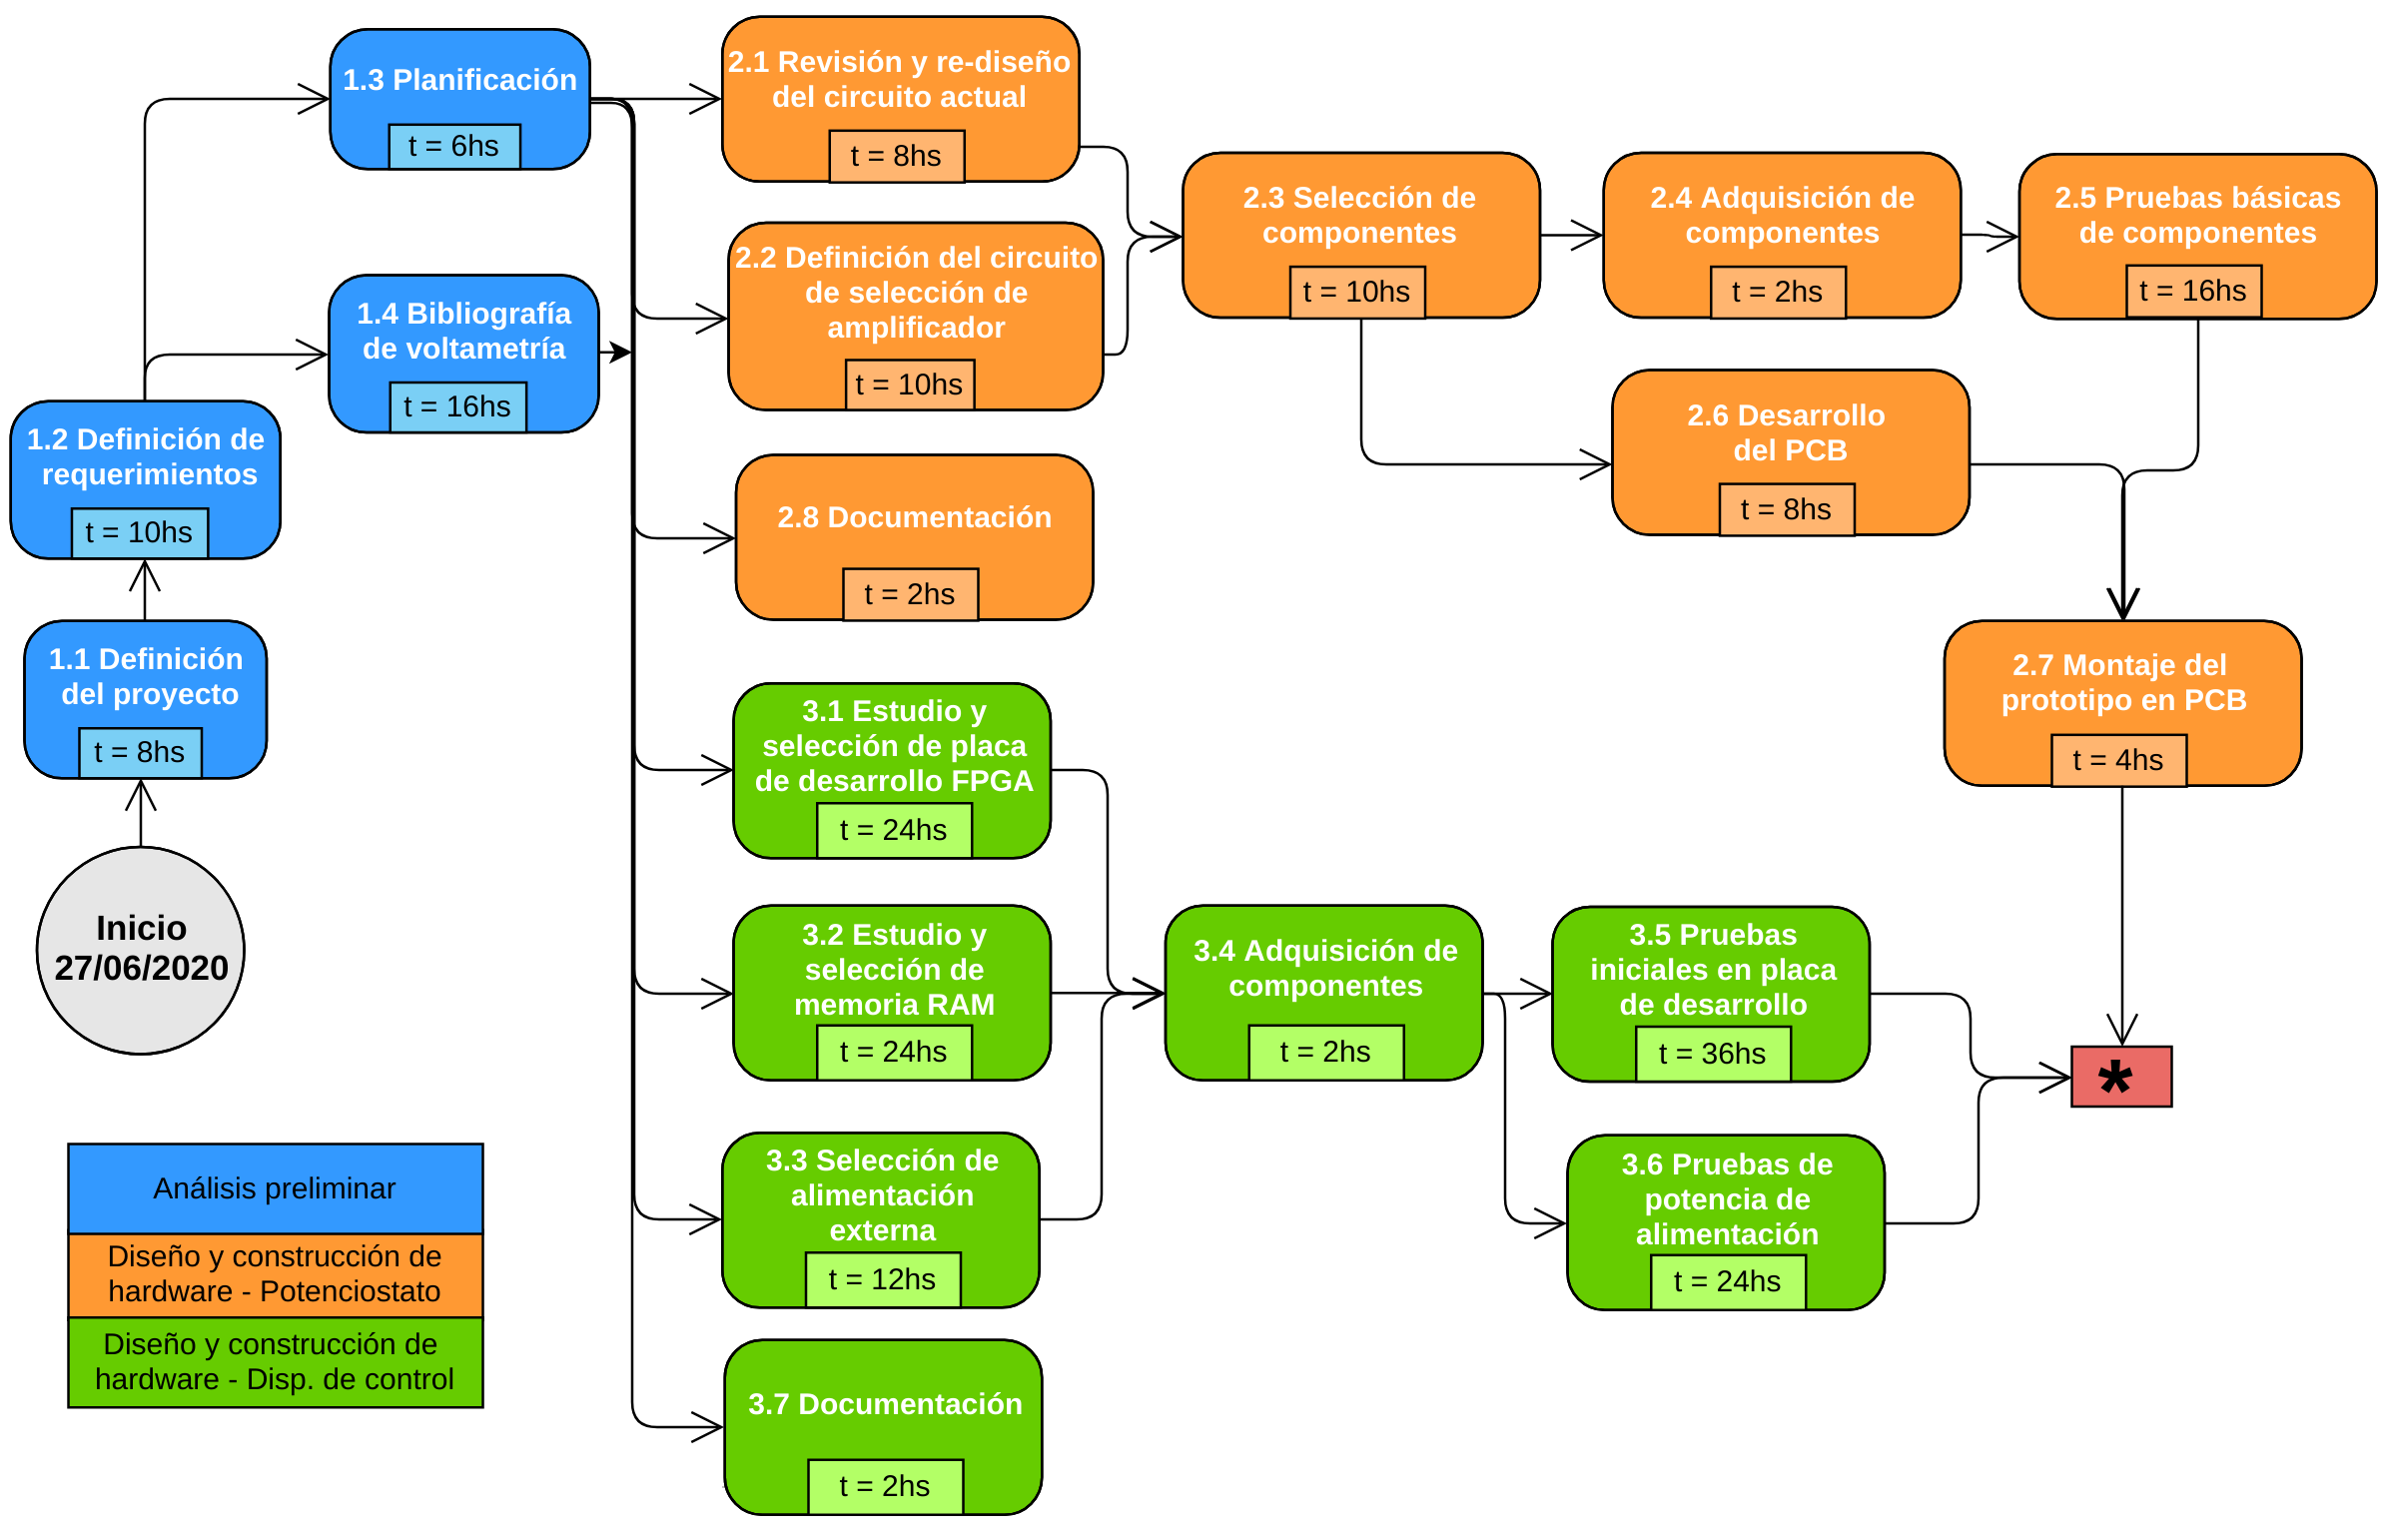
\includegraphics[width=1\textwidth]{./Figuras/Activity-On-Node1.png}
\caption{Diagrama en \textit{Activity on Node}. Primera parte}
\label{fig:AoN1}
\end{figure}

\begin{figure}[H]
\centering 
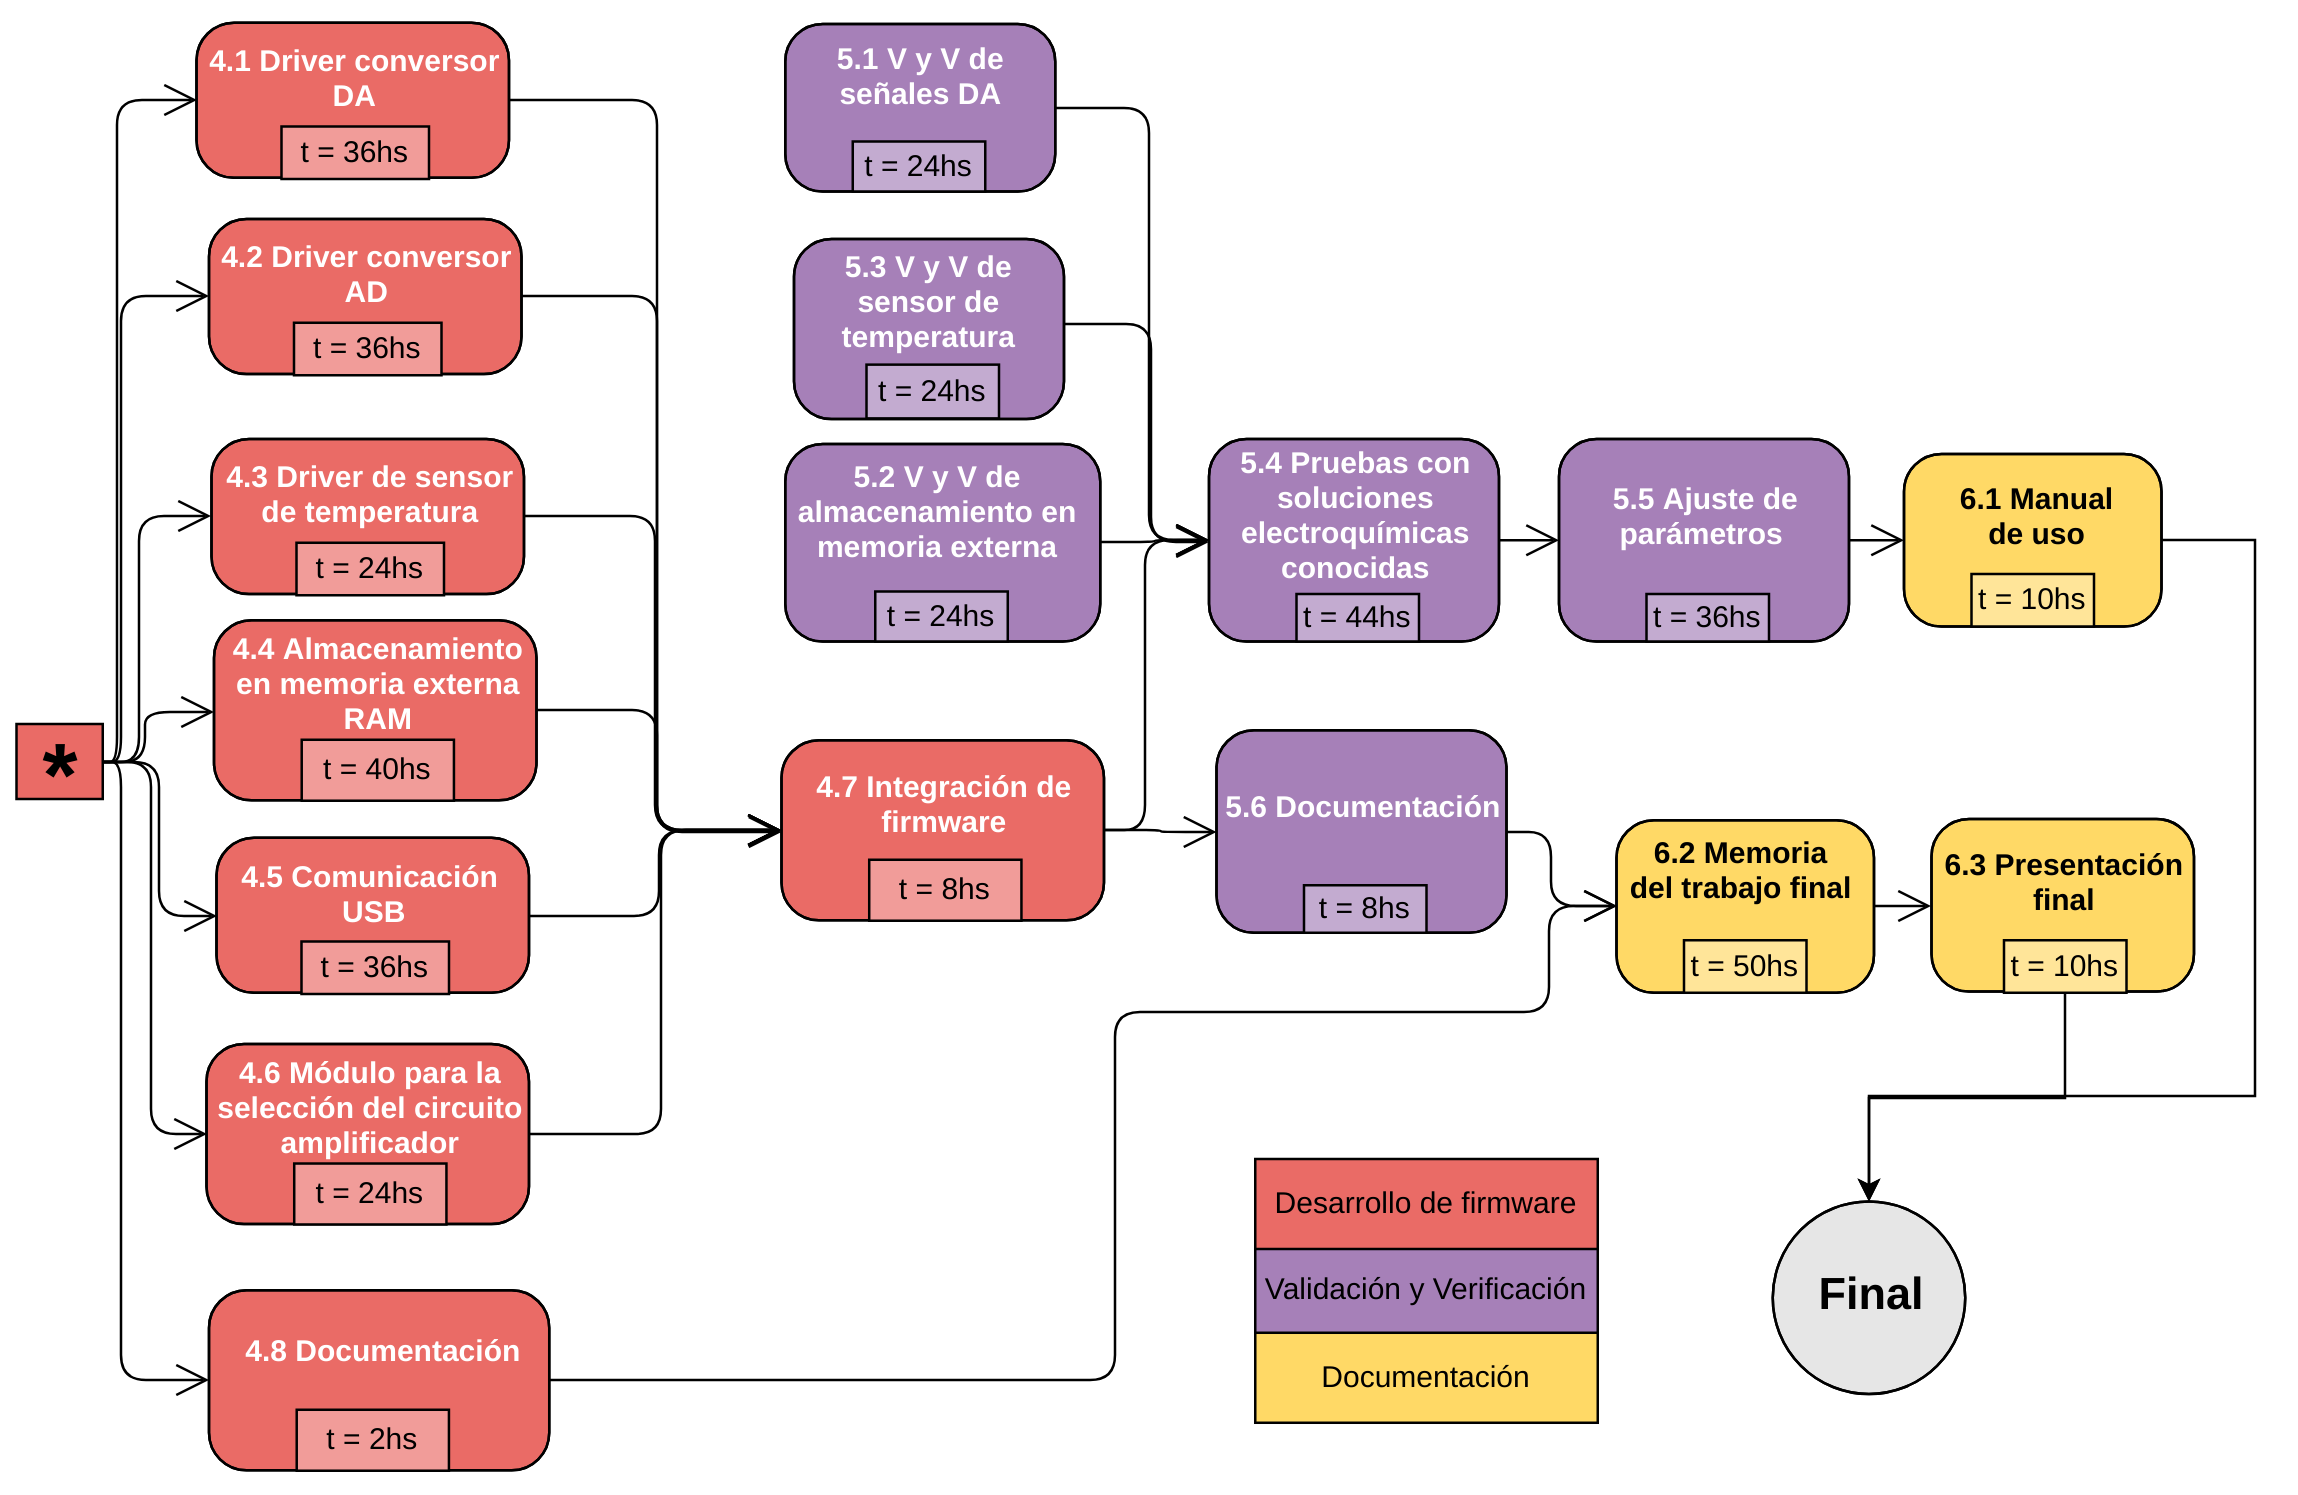
\includegraphics[width=1\textwidth]{./Figuras/Activity-On-Node2.png}
\caption{Diagrama en \textit{Activity on Node}. Segunda parte}
\label{fig:AoN2}
\end{figure}

\section{9. Diagrama de Gantt}
\label{sec:gantt}

\begin{figure}[H]
\centering 
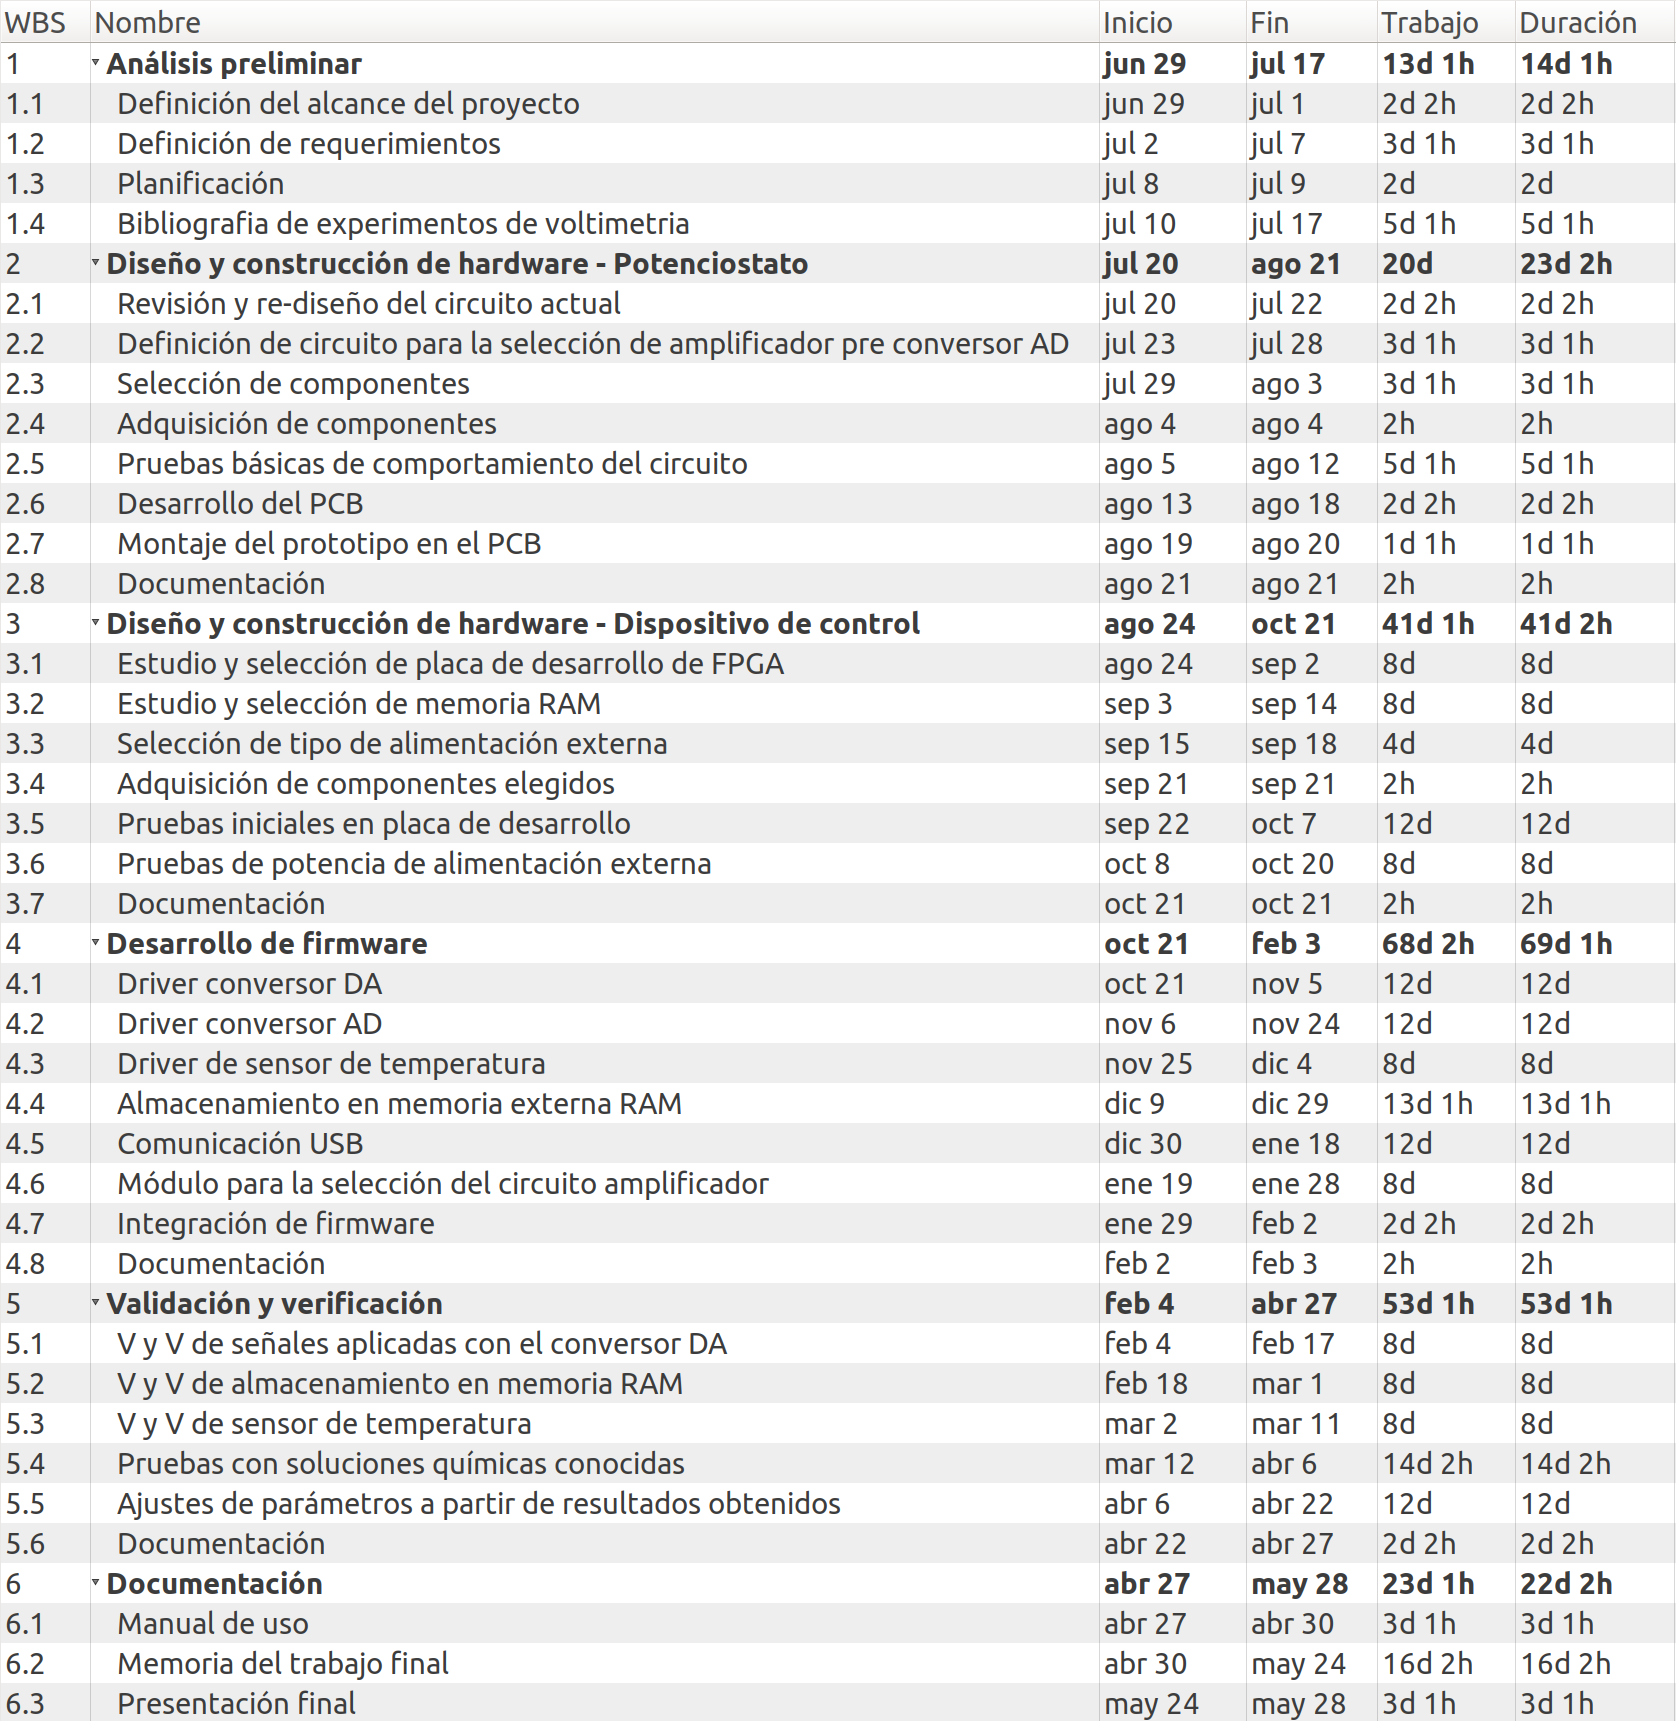
\includegraphics[width=1\textwidth]{./Figuras/tabla_gantt.png}
\caption{Tabla de tareas del diagrama gantt}
\label{fig:gantt_tabla}
\end{figure}
\begin{landscape}
\begin{figure}[H]
\centering 
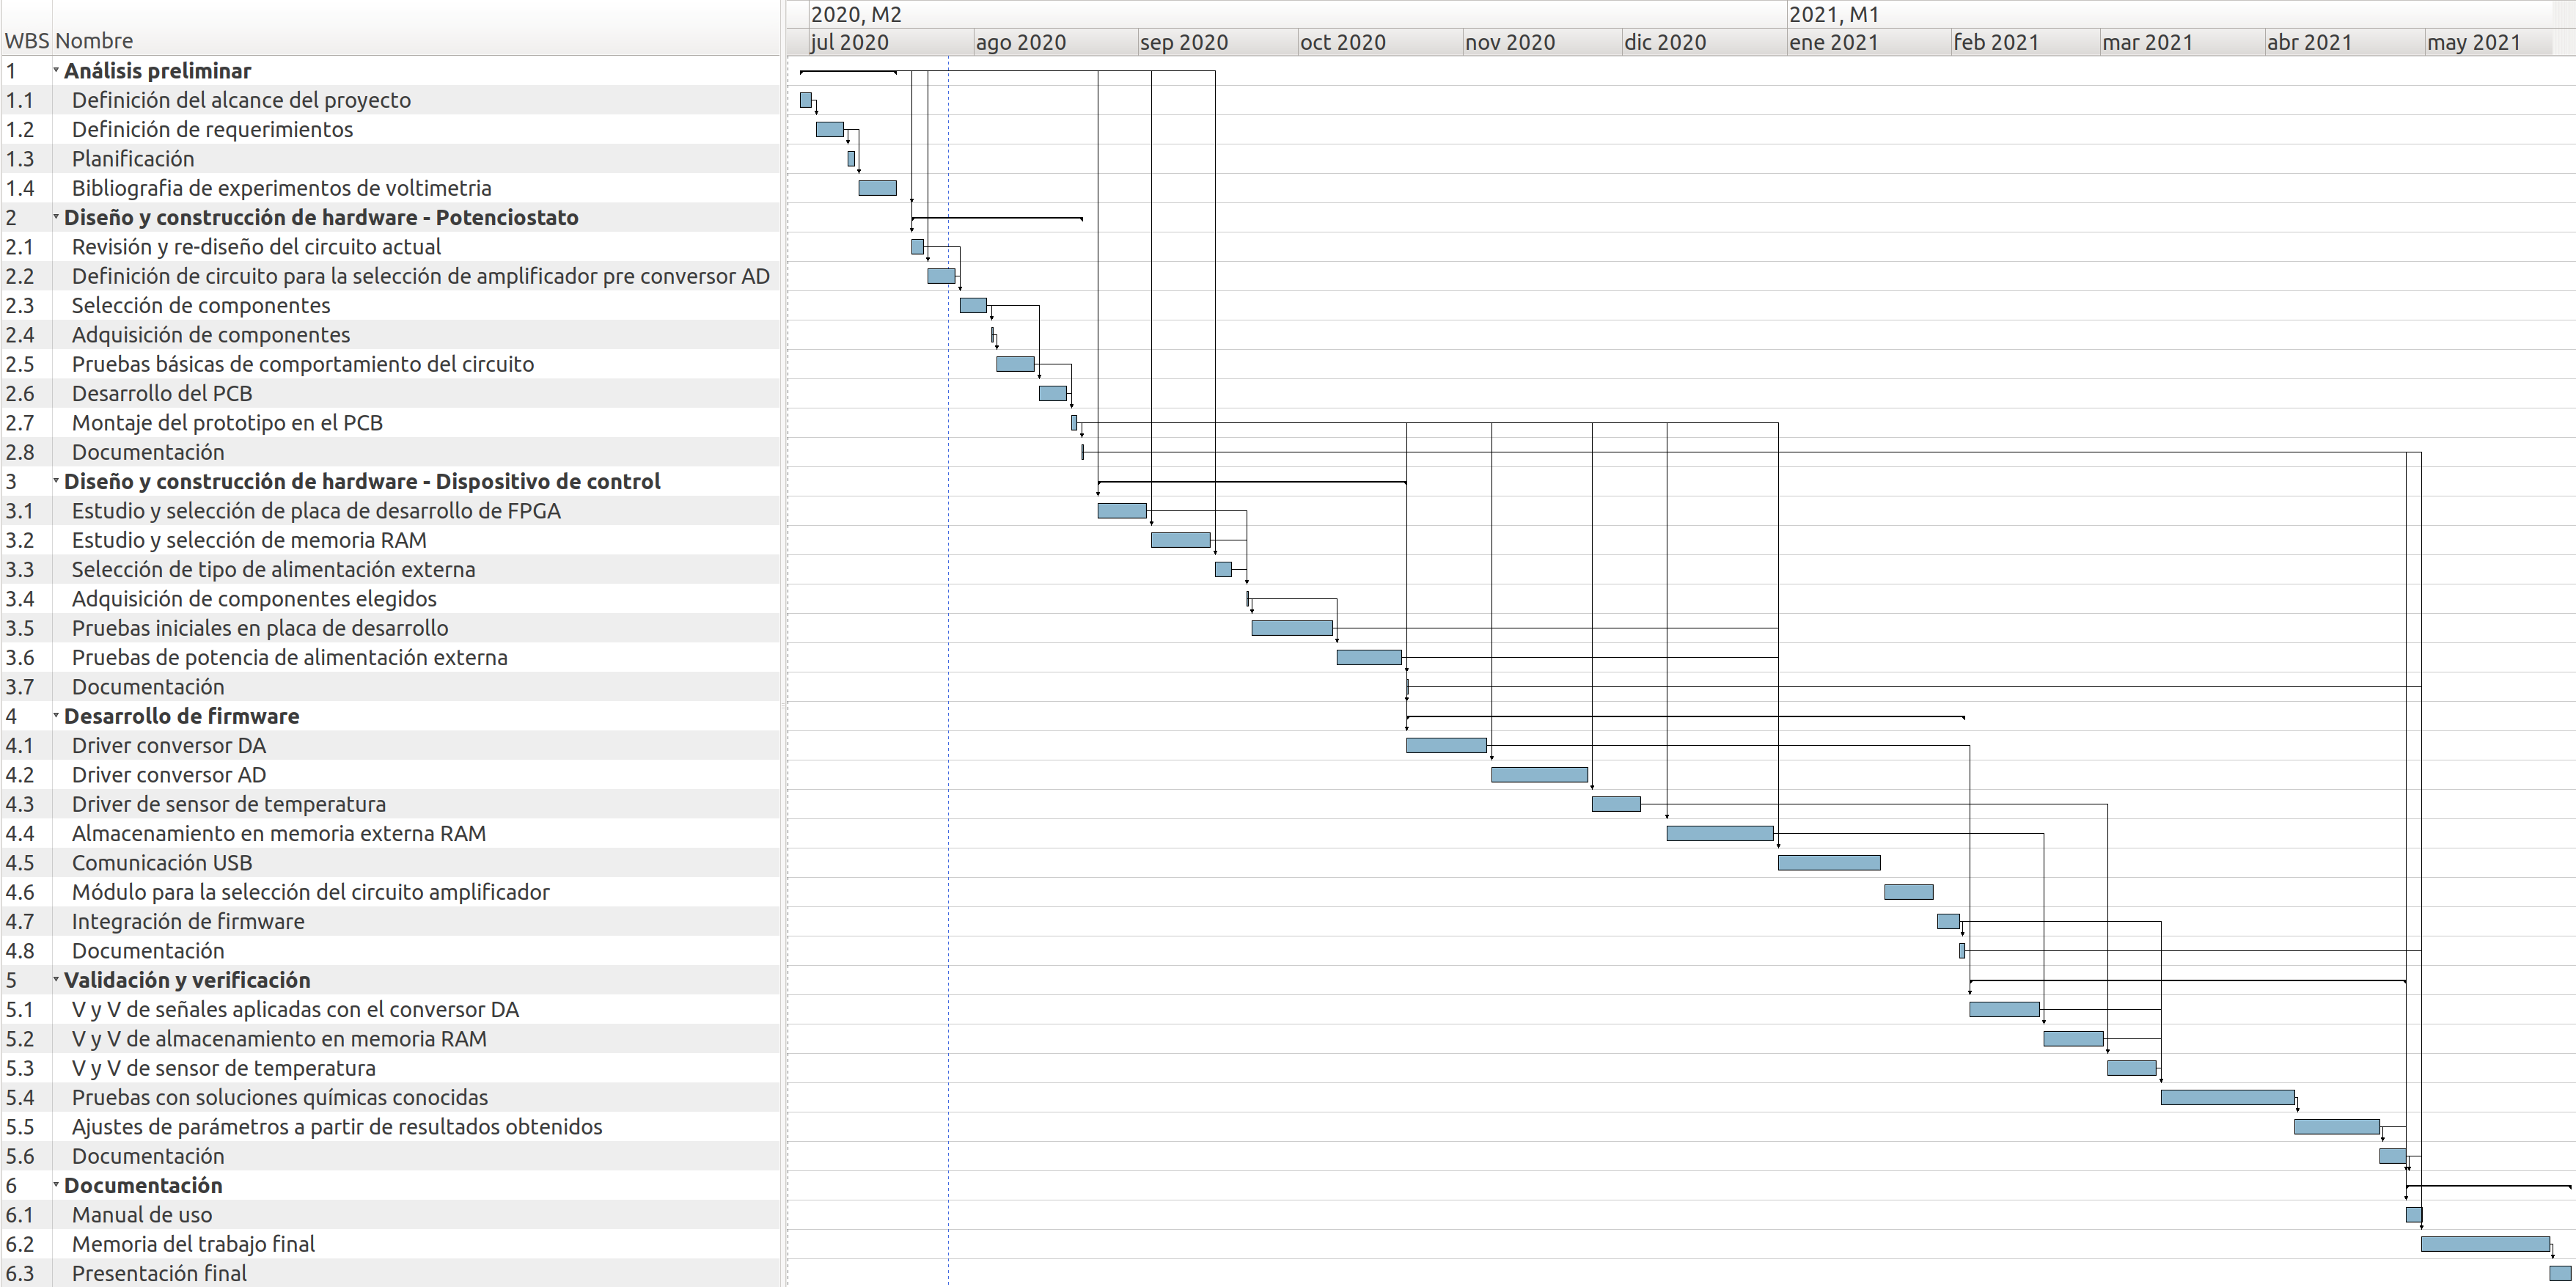
\includegraphics[width=1.6\textwidth]{./Figuras/gantt_full.png}
\caption{Diagrama de gantt}
\label{fig:gantt}
\end{figure}

\end{landscape}

\section{10. Matriz de uso de recursos de materiales}
\label{sec:recursos}

\begin{table}[H]
\label{tab:recursos}
\begin{tabular}{|c|c|c|c|c|c|}
\hline
\cellcolor[HTML]{C0C0C0} &
  \cellcolor[HTML]{C0C0C0} &
  \multicolumn{4}{c|}{\cellcolor[HTML]{C0C0C0}Recursos requeridos (horas)} \\ \cline{3-6} 
\multirow{-2}{*}{\cellcolor[HTML]{C0C0C0}Código WBS} &
  \multirow{-2}{*}{\cellcolor[HTML]{C0C0C0}Nombre Tarea} &
  \multicolumn{1}{l|}{PC} &
  \multicolumn{1}{l|}{FPGA} &
  \multicolumn{1}{l|}{Lab. electrónico} &
  \multicolumn{1}{l|}{Lab. químico} \\ \hline
1         & Análisis preliminar             & 40  & 0   & 0   & 0  \\ \hline
2         & Hardware - Potenciostato        & 44  & 0   & 0   & 0  \\ \hline
2.5       & Pruebas básicas del circuito    & 0   & 0   & 16  & 0  \\ \hline
2.7       & Montaje de prototipo            & 0   & 0   & 4   & 0  \\ \hline
3.1 - 3.4 & Dispositivo de control          & 62  & 0   & 0   & 0  \\ \hline
3.5       & Pruebas en FPGA                 & 0   & 36  & 0   & 0  \\ \hline
3.6       & Pruebas de alimentación         & 0   & 0   & 24  & 0  \\ \hline
4         & Desarrollo de firmware          & 206 & 206 & 0   & 0  \\ \hline
5         & Validación y verificación       & 0   & 116 & 116 & 0  \\ \hline
5.4       & Pruebas con soluciones químicas & 0   & 44  & 0   & 44 \\ \hline
6         & Documentación                   & 70  & 0   & 0   & 0  \\ \hline
\end{tabular}
\end{table}


\section{11. Presupuesto detallado del proyecto}
\label{sec:presupuesto}

\begin{table}[htpb]
\centering
\begin{tabularx}{\linewidth}{@{}|X|c|r|r|@{}}
\hline
\rowcolor[HTML]{C0C0C0} 
\multicolumn{4}{|c|}{\cellcolor[HTML]{C0C0C0}COSTOS DIRECTOS} \\ \hline
\rowcolor[HTML]{C0C0C0} 
Descripción &
  \multicolumn{1}{c|}{\cellcolor[HTML]{C0C0C0}Cantidad} &
  \multicolumn{1}{c|}{\cellcolor[HTML]{C0C0C0}Valor unitario} &
  \multicolumn{1}{c|}{\cellcolor[HTML]{C0C0C0}Valor total} \\ \hline
Componentes electrónicos potenciostato & 
  \multicolumn{1}{c|}{1} & 
  \multicolumn{1}{c|}{U\$S 110} &
  \multicolumn{1}{c|}{U\$S 110} \\ \hline
Placa de desarrollo FPGA &
  \multicolumn{1}{c|}{1} &
  \multicolumn{1}{c|}{U\$S 200} &
  \multicolumn{1}{c|}{U\$S 200} \\ \hline
Horas de ingeniería &
  \multicolumn{1}{c|}{660hs} &
  \multicolumn{1}{c|}{U\$S 10} &
  \multicolumn{1}{c|}{U\$S 6.600} \\ \hline
Soluciones químicas &  
  \multicolumn{1}{c|}{40} &
  \multicolumn{1}{c|}{U\$S 10} &
  \multicolumn{1}{c|}{U\$S 400} \\ \hline 
\multicolumn{3}{|c|}{SUBTOTAL} &
  \multicolumn{1}{c|}{U\$S 7.310} \\ \hline
\rowcolor[HTML]{C0C0C0} 
\hline
\multicolumn{4}{|c|}{\cellcolor[HTML]{C0C0C0}COSTOS INDIRECTOS} \\ \hline
\rowcolor[HTML]{C0C0C0} 
Descripción &
  \multicolumn{1}{c|}{\cellcolor[HTML]{C0C0C0}Cantidad} &
  \multicolumn{1}{c|}{\cellcolor[HTML]{C0C0C0}Valor unitario} &
  \multicolumn{1}{c|}{\cellcolor[HTML]{C0C0C0}Valor total} \\ \hline
30\% del total de los costos directos &
  \multicolumn{1}{c|}{1} &
  \multicolumn{1}{c|}{U\$S 2.193} &
  \multicolumn{1}{c|}{U\$S 2.193} \\ \hline 
\multicolumn{3}{|c|}{SUBTOTAL} &
  \multicolumn{1}{c|}{} \\ \hline
\rowcolor[HTML]{C0C0C0}
\multicolumn{3}{|c|}{TOTAL} &
 U\$S 9.503  \\ \hline
\end{tabularx}%
\end{table}


\section{12. Matriz de asignación de responsabilidades}
\label{sec:responsabilidades}

\begin{table}[H]
\centering
\resizebox{\linewidth}{!}{%
\begin{tabular}{|l|l|c|c|c|c|}
\hline
\rowcolor[HTML]{C0C0C0} 
\multicolumn{1}{|c|}{\cellcolor[HTML]{C0C0C0}} &
  \multicolumn{1}{c|}{\cellcolor[HTML]{C0C0C0}} &
  Responsable &
  Orientadores &
  Equipo &
  Cliente \\ \cline{3-6} 
\multicolumn{1}{|c|}{\multirow{-2}{*}{\cellcolor[HTML]{C0C0C0}\begin{tabular}[c]{@{}c@{}}Código \\ WBS\end{tabular}}} &
  \multicolumn{1}{c|}{\multirow{-2}{*}{\cellcolor[HTML]{C0C0C0}Nombre de la tarea}} &
  \begin{tabular}[c]{@{}c@{}}Fabiola \\ de las Casas Escardó\end{tabular} &
  \multicolumn{1}{l|}{\begin{tabular}[c]{@{}l@{}}Juan Manuel Reta\\ Eduardo Filomena\end{tabular}} &
  \multicolumn{1}{l|}{Iván G. Pollitzer} &
  \multicolumn{1}{l|}{Guido Rozenblum} \\ \hline
1 &
  Análisis preliminar & P & C & - &  S \\ \hline
2.1 &
  \begin{tabular}[c]{@{}l@{}}Revisión y re-diseño \\ del circuito actual\end{tabular} &  P & C & - & - \\ \hline
2.2 &
  \begin{tabular}[c]{@{}l@{}}Definición de circuito \\ de amplificación\end{tabular} &  P &  C & - & - \\ \hline
2.3 &  Selección de componentes &  P &  - & S & I \\ \hline
2.4 &
  Adquisición de componentes &  S & - &  P & A \\ \hline
2.5 &
  Pruebas básicas de circuito &  P & - & S & I \\ \hline
2.6 &
  Desarrollo PCB & P & - & - & - \\ \hline
2.7 &
  Montaje de prototipo en PCB &  S & - &  P & - \\ \hline
3.1 &
  Estudio y selección de FPGA &  P & C & I & - \\ \hline
3.2 &
  Estudio y selección de RAM &  P & C & I & - \\ \hline
3.3 &
  Selección alimentación externa & P & C & I & - \\ \hline
3.4 &
  Adquisición de componentes & S & - & P & A \\ \hline
3.5 &
  Pruebas iniciales con FPGA & P & C & - & - \\ \hline
3.6 &
  \begin{tabular}[c]{@{}l@{}}Pruebas de potencia de \\ alimentación externa\end{tabular} &  P & C & - & - \\ \hline
4 &
  Desarrollo de firmware & P & C & S & - \\ \hline
5.1 &
  \begin{tabular}[c]{@{}l@{}}V y V de señales del \\ conversor DA\end{tabular} &
  P & I & S & C / A \\ \hline
5.2 &
  \begin{tabular}[c]{@{}l@{}}V y V de almacenamiento \\ en RAM\end{tabular} &
  P &  I & S & A \\ \hline
5.3 &
  \begin{tabular}[c]{@{}l@{}}V y V de sensor de \\ temperatura\end{tabular} &
  P & I & S & C / A \\ \hline
5.4 &
  \begin{tabular}[c]{@{}l@{}}Pruebas con soluciones \\ electroquímicas conocidas\end{tabular} & P & I & S & S \\ \hline
5.5 &
  Ajustes de parámetros & P & C & S & A \\ \hline
6 &
  Documentación & P & C / A & - & I \\ \hline
\end{tabular}%
}
\end{table}

{\footnotesize
Referencias:
\begin{itemize}
	\item P = Responsabilidad Primaria
	\item S = Responsabilidad Secundaria
	\item A = Aprobación
	\item I = Informado
	\item C = Consultado
\end{itemize}
} %footnotesize

\section{13. Gestión de riesgos}
\label{sec:riesgos}

\textbf{Riesgo 1:} Imposibilidad para cumplir los plazos del proyecto.
\begin{itemize}
\item Severidad (S): 8, retrasaría la entrega del prototipo funcional al cliente.
\item Probabilidad de ocurrencia (O): 3, la empresa brindará soporte alivianando la carga de otros proyectos del responsable.
\end{itemize}

\textbf{Riesgo 2:} Errores en el diseño del prototipo
\begin{itemize}
\item Severidad (S): 9, genera retrasos y un aumento de costos.
\item Probabilidad de ocurrencia (O): 7, hay tener en cuenta muchas especificaciones de las distintas partes del prototipo.
\end{itemize}

\textbf{Riesgo 3:} Demoras en la importación de componentes.
\begin{itemize}
\item Severidad (S): 8, genera un retraso general 
\item Probabilidad de ocurrencia (O): 8, debido a la situación actual (pandemia CoVID-19) hay mucha incerteza con lo relacionado a la importación.
\end{itemize}

\textbf{Riesgo 4:} Demora y complejidad de los ensayos electroquímicos
\begin{itemize}
\item Severidad (S): 7, no se lograria validar el funcionamiento final del proyecto.
\item Probabilidad de ocurrencia (O): 4, actualmente ya se están realizando algunos experimentos, por lo que se tiene la experiencia y apoyo suficiente para diminuir este riesgo.
\end{itemize}

\textbf{Riesgo 5:} Cambio de especificaciones por parte del cliente
\begin{itemize}
\item Severidad (S): 7, dependiendo que especificación se pida modificar el riesgo puede ser menor.
\item Probabilidad de ocurrencia (O): 7, al ser un producto para realizar mediciones electroquimicas nuevas, no se conoce con demasiada presicion las verdaderas necesidades del prototipo final.
\end{itemize}

b) Tabla de gestión de riesgos:      (El RPN se calcula como RPN=SxO)

\begin{table}[H]
\centering
\begin{tabular}{|c|c|c|c|c|c|c|}
\hline
\rowcolor[HTML]{C0C0C0} 
Riesgo & S & O & RPN & S* & O* & RPN* \\ \hline
1      & 8 & 3 & 24  & -  &  - & -    \\ \hline
2      & 9 & 7 & 63  & 7  & 5  & 35   \\ \hline
3      & 8 & 8 & 64  & 6  & 7  & 42     \\ \hline
4      & 7 & 4 & 28  & -  & -  &      \\ \hline
5      & 7 & 7 & 49  & 6  & 5  & 30   \\ \hline
\end{tabular}
\end{table}

Criterio adoptado: 
Se tomarán medidas de mitigación en los riesgos cuyos números de RPN sean mayores a 45.

Nota: los valores marcados con (*) en la tabla corresponden luego de haber aplicado la mitigación.

c) Plan de mitigación de los riesgos que originalmente excedían el RPN máximo establecido:

Riesgo 2: se realizarán consultas y validaciones del diseño al director y co-director. Además el prototipo se realizará en módulos acoplables y de esta manera, si hay un error de diseño solo será necesario cambiar dicho modulo.
\begin{itemize}
\item Severidad (S*): 7, se verá afectado solo el modulo con el error por lo que se podrá continuar con el resto del proyecto, mientras se fábrica nuevamente dicho modulo corregido.
\item Probabilidad de ocurrencia (O*): 5, al tener revisiones periódicas con el director y co-director aumenta al probabilidad de detectar estos errores con tiempo.
\end{itemize}
Riesgo 3: se buscarán proveedores locales y en caso de no haber, se aumentará la cantidad de cada componente pedido al exterior. De esta forma, en caso de haber demora solo se producirá en ese único pedido.
\begin{itemize}
\item Severidad (S*): 6, las proveedores locales disponen de la mayoría de los componentes requeridos, pero a un precio mayor en algunos casos.
\item Probabilidad de ocurrencia (O*): 7, el contexto actual excede una previsión precisa y hay componentes que solo se consiguen en el exterior.
\end{itemize}
Riesgo 5: se extenderán los rangos máximos de los distintos experimentos a realizar, basado en bibliografía existente, y se incluirán las prestaciones de los equipos disponibles en el mercado, confirmando con el cliente todas las definiciones.
\begin{itemize}
\item Severidad (S*): 6, al ampliar las prestaciones y rangos de medición pedidos por el cliente se anticipan posibles cambios futuros.
\item Probabilidad de ocurrencia (O*): 5, el cliente siempre puede buscar cambiar las especificaciones pero al haber confirmado todo previo al comienzo del proyecto ya esta al tanto de las limitaciones del mismo.
\end{itemize}

\section{14. Gestión de la calidad}
\label{sec:calidad}

\begin{itemize}
\item \textbf{Req \#1.1:} Debe poder controlarse mediante USB 3.1.

Verificación y validación:
\begin{itemize}
\item Verificación: se conectará a una PC con USB 3.1 y se harán pruebas de recepción y envío de datos.
\item Validación: el cliente probará esta comunicación con la PC a utilizar por la empresa.
\end{itemize}

\item\textbf{ Req. \#2.1 y \#2.2:} Se deben poder medir corrientes en el rango de 1 pA hasta los 100 nA. Rango previamente definido por el usuario. Y el error de las mediciones, una vez seleccionado el rango de corriente, debe ser menor al 10\%.

Verificación y validación:
\begin{itemize}
\item Verificación: Se armará un banco de pruebas con una fuente de corriente con dichos rangos y se conectará la señal de corriente conocida a los electrodos. Se extraen los datos leído por el ADC y se analizarán en un programa realizado en Python.
\item Validación: Se realizarán pruebas con soluciones químicas cuya reacción electroquímica es conocida. Se analizarán los datos recibidos y se compararán los resultados con los obtenidos en un potenciostato comercial.
\end{itemize}

\item \textbf{Req. \#2.3:} Todos los electrodos se tienen que poder medir en 1,6 ms o a una frecuencia de 625Hz.

Verificación y validación:
\begin{itemize}
\item Verificación: Se medirá el tiempo de ejecución de la adquisición de datos y almacenamiento del mismo.
\item Validación: Se realizará un experimento electroquímico conocido y se mostrarán el intervalo de tiempo en que se obtuvieron los datos obtenidos de todos los electrodos en simultáneo
\end{itemize}

\item \textbf{Req. \#2.4:} Se debe poder seleccionar si medir mínimos y máximos o tomar mediciones en intervalos de tiempo constantes y definidos por el usuario.

Verificación y validación:
\begin{itemize}
\item Verificación: Se definirán en el firmware el experimento a realizar y con una fuente de corriente aplicada en un electrodo se verificará que los datos adquiridos con el ADC corresponden a los definidos.
\item Validación: Se realizará un experimento electroquímico conocido y se mostrarán los datos obtenidos con el ADC de un electrodo corresponde a los valores pedidos (mínimo, máximo, intervalo de tiempo).
\end{itemize}

\item \textbf{Req. \#3.1, \#3.2 y \#3.3:} Requerimientos de voltametría.

Verificación y validación:
\begin{itemize}
\item Verificación: Se configura la señal a generar por el DAC y se mide con un osciloscopio que dicha señal tenga las características configuradas.
\item Validación: Se realizará un experimento electroquímico conocido y se medirá con un osciloscopio que la señal aplicada al CE tiene las especificaciones seleccionadas..
\end{itemize}

\end{itemize}


\section{15. Comunicación del proyecto}
\label{sec:comunicaciones}

\begin{table}[H]
\centering
\resizebox{\textwidth}{!}{%
\begin{tabular}{|c|l|l|l|l|l|}
\hline
\rowcolor[HTML]{C0C0C0} 
\multicolumn{6}{|c|}{\cellcolor[HTML]{C0C0C0}PLAN DE COMUNICACIÓN DEL PROYECTO} \\ \hline
\rowcolor[HTML]{C0C0C0} 
¿Qué comunicar? &
  \multicolumn{1}{c|}{\cellcolor[HTML]{C0C0C0}Audiencia} &
  \multicolumn{1}{c|}{\cellcolor[HTML]{C0C0C0}Propósito} &
  \multicolumn{1}{c|}{\cellcolor[HTML]{C0C0C0}Frecuencia} &
  \multicolumn{1}{c|}{\cellcolor[HTML]{C0C0C0}Método de comunicac.} &
  \multicolumn{1}{c|}{\cellcolor[HTML]{C0C0C0}Responsable} \\ \hline
Plan de trabajo &
  \begin{tabular}[c]{@{}l@{}}Todos los\\ interesados\end{tabular} &
  \begin{tabular}[c]{@{}l@{}}Informar del alcance \\ del proyecto\end{tabular} &
  Una vez &
  Reunión online &
  \begin{tabular}[c]{@{}l@{}}Fabiola de las \\ Casas Escardó\end{tabular} \\ \hline
Avance del trabajo &
  \begin{tabular}[c]{@{}l@{}}Director\\ Co-director\end{tabular} &
  \begin{tabular}[c]{@{}l@{}}Informar y validar el \\ progreso\end{tabular} &
  15 días &
  Reuniones online &
  \begin{tabular}[c]{@{}l@{}}Fabiola de las \\ Casas Escardó\end{tabular} \\ \hline
Consultas &
  \begin{tabular}[c]{@{}l@{}}Director\\ Co-director\end{tabular} &
  \begin{tabular}[c]{@{}l@{}}Sugerencias y \\ búsqueda de soluciones\end{tabular} &
  15 días &
  Reuniones online &
  \begin{tabular}[c]{@{}l@{}}Fabiola de las \\ Casas Escardó\end{tabular} \\ \hline
Pruebas de aceptación &
  Cliente &
  \begin{tabular}[c]{@{}l@{}}Validación del \\ prototipo\end{tabular} &
  \begin{tabular}[c]{@{}l@{}}Al finalizar el \\ prototipo\end{tabular} &
  Reunión presencial &
  \begin{tabular}[c]{@{}l@{}}Fabiola de las \\ Casas Escardó\end{tabular} \\ \hline
Finalización del proyecto &
  \begin{tabular}[c]{@{}l@{}}Todos los\\ interesados\end{tabular} &
  Conocer los resultados &
  \begin{tabular}[c]{@{}l@{}}Al finalizar\\ el proyecto\end{tabular} &
  Reunión online &
  \begin{tabular}[c]{@{}l@{}}Fabiola de las \\ Casas Escardó\end{tabular} \\ \hline
\end{tabular}
}%
\end{table}


\section{16. Gestión de Compras}
\label{sec:compras}

Como se indicó en la matriz de asignación de responsabilidades las compras serán realizadas por otro integrante de la empresa. Por lo que los proveedores de los componentes electrónicos necesarios y la empresa encargada de la fabricación del PCB serán seleccionados por dicha persona.
 
\section{17. Seguimiento y control}
\label{sec:seguimiento}

\begin{table}[H]
\centering
\begin{tabular}{|c|l|l|l|l|l|}
\hline
\rowcolor[HTML]{C0C0C0} 
\multicolumn{6}{|c|}{\cellcolor[HTML]{C0C0C0}SEGUIMIENTO DE AVANCE} \\ \hline
\rowcolor[HTML]{C0C0C0} 
\begin{tabular}[c]{@{}c@{}}Tarea del \\ WBS\end{tabular} &
  \multicolumn{1}{c|}{\cellcolor[HTML]{C0C0C0}\begin{tabular}[c]{@{}c@{}}Indicador de \\ avance\end{tabular}} &
  \multicolumn{1}{c|}{\cellcolor[HTML]{C0C0C0}\begin{tabular}[c]{@{}c@{}}Frecuencia \\ de reporte\end{tabular}} &
  \multicolumn{1}{c|}{\cellcolor[HTML]{C0C0C0}\begin{tabular}[c]{@{}c@{}}Resp. de \\ seguimiento\end{tabular}} &
  \multicolumn{1}{c|}{\cellcolor[HTML]{C0C0C0}\begin{tabular}[c]{@{}c@{}}Persona a ser \\ informada\end{tabular}} &
  \multicolumn{1}{c|}{\cellcolor[HTML]{C0C0C0}\begin{tabular}[c]{@{}c@{}}Método \\ comunic.\end{tabular}} \\ \hline
1.1 y 1.2 &
  \begin{tabular}[c]{@{}l@{}}Reporte de \\ definición\end{tabular} &
  Una vez &
  \begin{tabular}[c]{@{}l@{}}Fabiola de las \\ Casas Escardó\end{tabular} &
  \begin{tabular}[c]{@{}l@{}}Juan Manuel Reta\\ Eduardo Filomena\end{tabular} &
  \begin{tabular}[c]{@{}l@{}}Correo \\ electrónico\end{tabular} \\ \hline
\rowcolor[HTML]{EFEFEF} 
1.3 &
  \begin{tabular}[c]{@{}l@{}}Entregas \\ parciales y \\ final del \\ documento\end{tabular} &
  \begin{tabular}[c]{@{}l@{}}Una vez por \\ semana mientras \\ dure la tarea\end{tabular} &
  \begin{tabular}[c]{@{}l@{}}Fabiola de las\\ Casas Escardó\end{tabular} &
  \begin{tabular}[c]{@{}l@{}}Juan Manuel Reta\\ Eduardo Filomena\\ Ariel Lutenberg\\ Patricio Bos\end{tabular} &
  \begin{tabular}[c]{@{}l@{}}Correo \\ electrónico\end{tabular} \\ \hline
2.1 y 2.2 &
  \begin{tabular}[c]{@{}l@{}}Reporte de \\ definición\end{tabular} &
  2 veces &
  \begin{tabular}[c]{@{}l@{}}Fabiola de las \\ Casas Escardó\end{tabular} &
  \begin{tabular}[c]{@{}l@{}}Juan Manuel Reta\\ Eduardo Filomena\end{tabular} &
  \begin{tabular}[c]{@{}l@{}}Correo \\ electrónico\end{tabular} \\ \hline
\rowcolor[HTML]{EFEFEF} 
2.3 - 2.8 &
  \begin{tabular}[c]{@{}l@{}}Reporte de \\ avance\end{tabular} &
  \begin{tabular}[c]{@{}l@{}}Cada 15 días hasta \\ terminar la tarea\end{tabular} &
  \begin{tabular}[c]{@{}l@{}}Fabiola de las \\ Casas Escardó\end{tabular} &
  \begin{tabular}[c]{@{}l@{}}Juan Manuel Reta\\ Eduardo Filomena\end{tabular} &
  \begin{tabular}[c]{@{}l@{}}Correo \\ electrónico\end{tabular} \\ \hline
3.1 - 3.4 &
  \begin{tabular}[c]{@{}l@{}}Reporte de \\ avance\end{tabular} &
  \begin{tabular}[c]{@{}l@{}}Cada 15 días hasta \\ terminar la tarea\end{tabular} &
  \begin{tabular}[c]{@{}l@{}}Fabiola de las \\ Casas Escardó\end{tabular} &
  \begin{tabular}[c]{@{}l@{}}Juan Manuel Reta\\ Eduardo Filomena\end{tabular} &
  \begin{tabular}[c]{@{}l@{}}Correo \\ electrónico\end{tabular} \\ \hline
\rowcolor[HTML]{EFEFEF} 
3.5 y 3.6 &
  \begin{tabular}[c]{@{}l@{}}Reporte de \\ resultados\\ obtenidos\end{tabular} &
  \begin{tabular}[c]{@{}l@{}}Cada 7 días hasta \\ terminar la tarea\end{tabular} &
  \begin{tabular}[c]{@{}l@{}}Fabiola de las \\ Casas Escardó\end{tabular} &
  \begin{tabular}[c]{@{}l@{}}Juan Manuel Reta\\ Eduardo Filomena\end{tabular} &
  \begin{tabular}[c]{@{}l@{}}Correo \\ electrónico\end{tabular} \\ \hline
4 &
  \begin{tabular}[c]{@{}l@{}}Drivers y \\ modulos \\ funcionando\end{tabular} &
  \begin{tabular}[c]{@{}l@{}}Cada 15 días hasta \\ terminar la tarea\end{tabular} &
  \begin{tabular}[c]{@{}l@{}}Fabiola de las \\ Casas Escardó\end{tabular} &
  \begin{tabular}[c]{@{}l@{}}Juan Manuel Reta\\ Eduardo Filomena\end{tabular} &
  \begin{tabular}[c]{@{}l@{}}Correo \\ electrónico\end{tabular} \\ \hline
\rowcolor[HTML]{EFEFEF} 
5.1 &
  \begin{tabular}[c]{@{}l@{}}Reporte de \\ resultados\\ obtenidos\end{tabular} &
  \begin{tabular}[c]{@{}l@{}}Cada 15 días hasta \\ terminar la tarea\end{tabular} &
  \begin{tabular}[c]{@{}l@{}}Fabiola de las \\ Casas Escardó\end{tabular} &
  \begin{tabular}[c]{@{}l@{}}Juan Manuel Reta\\ Eduardo Filomena\\ Guido Ronzenblum\end{tabular} &
  \begin{tabular}[c]{@{}l@{}}Correo \\ electrónico\end{tabular} \\ \hline
5.2 &
  \begin{tabular}[c]{@{}l@{}}Reporte de \\ resultados \\ obtenidos\end{tabular} &
  \begin{tabular}[c]{@{}l@{}}Cada 15 días hasta \\ terminar la tarea\end{tabular} &
  \begin{tabular}[c]{@{}l@{}}Fabiola de las \\ Casas Escardó\end{tabular} &
  \begin{tabular}[c]{@{}l@{}}Juan Manuel Reta\\ Eduardo Filomena\\ Guido Ronzenblum\end{tabular} &
  \begin{tabular}[c]{@{}l@{}}Correo \\ electrónico\end{tabular} \\ \hline
\rowcolor[HTML]{EFEFEF} 
5.3 &
  \begin{tabular}[c]{@{}l@{}}Reporte de \\ resultados \\ obtenidos\end{tabular} &
  \begin{tabular}[c]{@{}l@{}}Cada 15 días hasta\\ terminar la tarea\end{tabular} &
  \begin{tabular}[c]{@{}l@{}}Fabiola de las \\ Casas Escardó\end{tabular} &
  \begin{tabular}[c]{@{}l@{}}Juan Manuel Reta\\ Eduardo Filomena\\ Guido Ronzenblum\end{tabular} &
  \begin{tabular}[c]{@{}l@{}}Correo \\ electrónico\end{tabular} \\ \hline
5.4 y 5.5 &
  \begin{tabular}[c]{@{}l@{}}Reporte de \\ resultados \\ obtenidos\end{tabular} &
  \begin{tabular}[c]{@{}l@{}}Cada 15 días hasta \\ terminar la tarea\end{tabular} &
  \begin{tabular}[c]{@{}l@{}}Fabiola de las \\ Casas Escardó\end{tabular} &
  \begin{tabular}[c]{@{}l@{}}Juan Manuel Reta\\ Eduardo Filomena\\ Guido Ronzenblum\end{tabular} &
  \begin{tabular}[c]{@{}l@{}}Correo \\ electrónico\end{tabular} \\ \hline
\rowcolor[HTML]{EFEFEF} 
6 &
  \begin{tabular}[c]{@{}l@{}}Secciones del \\ informe \\ realizadas.\end{tabular} &
  \begin{tabular}[c]{@{}l@{}}Cada 15 días hasta \\ terminar la tarea\end{tabular} &
  \begin{tabular}[c]{@{}l@{}}Fabiola de las \\ Casas Escardó\end{tabular} &
  \begin{tabular}[c]{@{}l@{}}Juan Manuel Reta\\ Eduardo Filomena\end{tabular} &
  \begin{tabular}[c]{@{}l@{}}Correo \\ electrónico\end{tabular} \\ \hline
\end{tabular}
\end{table}

\section{18. Procesos de cierre}    
\label{sec:cierre}

\begin{itemize}

\item Pautas de trabajo que se seguirán para analizar si se respetó el Plan de Proyecto original, a cargo de la Ing. \authorname
\begin{itemize}
\item Evaluación de las tareas y los tiempos: se armará una tabla en la cual se comparará las tareas propuestas con las realizadas y los tiempos propuestos con los reales. Se calculará el desvío y las causas de dicho desvío, si lo hubo.
\item Evaluación de costos: se analizará el costo inicial del proyecto y el costo real a la finalización. Si hay diferencias, se evaluará en que puntos se produjeron y debido a qué. 
\end{itemize}

\item Se realizará un informe identificando las técnicas y procedimientos útiles e inútiles que se utilizaron, y los problemas que surgieron y cómo se solucionaron, a cargo de la Ing. \authorname

\item Se invitará a la presentación pública del proyecto final a todas las personas colaboradoras del proyecto. En dicha presentación se agradecerá al director y al co-director del proyecto, así como a los jurados, compañeros, docentes y autoridades de la Carrera de Especialización en Sistemas Embebidos, y a los integrantes de la empresa Aplife Biotech S.A. por su colaboración y apoyo. 

\end{itemize}

\end{document}
